%%
%% Style file "borrowed" from Michel Goemans
%%
\documentclass[11pt]{article}

\usepackage{url,amsmath,amsthm,amsfonts,amssymb}
\usepackage{pgf}

\def\ceil#1{\lceil #1 \rceil}
\def\floor#1{\lfloor #1 \rfloor}
\def\ang#1{\langle #1 \rangle}

\newtheorem{definition}{Definition}
\newtheorem{remark}{Remark}
\newtheorem{theorem}{Theorem}
\newtheorem{lemma}[theorem]{Lemma}
\newtheorem{corollary}[theorem]{Corollary}
\newtheorem{proposition}[theorem]{Proposition}
\newtheorem{claim}[theorem]{Claim}
\newtheorem{observation}{Observation}

\newcommand{\R}{{\mathbb R}}
\newcommand{\Var}{\hbox{Var}}
\newcommand{\Z}{{\mathbb Z}}
\newcommand{\Q}{{\mathbb Q}}
\newcommand{\C}{{\mathbb C}}
\newcommand{\N}{{\mathbb N}}

\newlength{\toppush}
\setlength{\toppush}{2\headheight}
\addtolength{\toppush}{\headsep}

\newcommand{\htitle}[2]{\noindent\vspace*{-\toppush}\newline\parbox{6.5in}
 {\large Addis Ababa University, Amist Kilo \hfill #1\newline
\hspace*{\fill}{\bf Algorithms and Programming for High Schoolers} \hspace*{\fill} \newline
\mbox{}\hrulefill\mbox{}}\vspace*{1ex}\mbox{}\newline
\begin{center}{\Large\bf #2}\end{center}}

\newcommand{\handout}[3]{\thispagestyle{empty}
 \markboth{ #2}{ #2}
 \pagestyle{myheadings}\htitle{\protect\ref{#1}}{#2}{#3}}

\setlength{\oddsidemargin}{0pt}
\setlength{\evensidemargin}{0pt}
\setlength{\textwidth}{6.5in}
\setlength{\topmargin}{0in}
\setlength{\textheight}{8.5in}

\newcommand{\eps}{\varepsilon}
\newcommand{\sq}[1]{\langle#1\rangle}

\begin{document}

\htitle{July 26, 2016}{Lecture 7}

\paragraph{\Large Memoization:}

Memoization is recursion, but where you remember answers that you have
computed before.  For many problems, this allows trading a small
amount of extra memory
usage (to store previously seen answers) to have significant gains in
running time.
Recall our code from lecture 3 to compute the $n$th
Fibonacci number.

\begin{verbatim}
def fibonacci(n):
    if n<2:
        return 1
    return fibonacci(n-1) + fibonacci(n-2)
\end{verbatim}

The recursion tree for computing \texttt{fibonacci}(5) looks as
follows.

\begin{figure}[!!h]
\begin{center}
\scalebox{0.4}{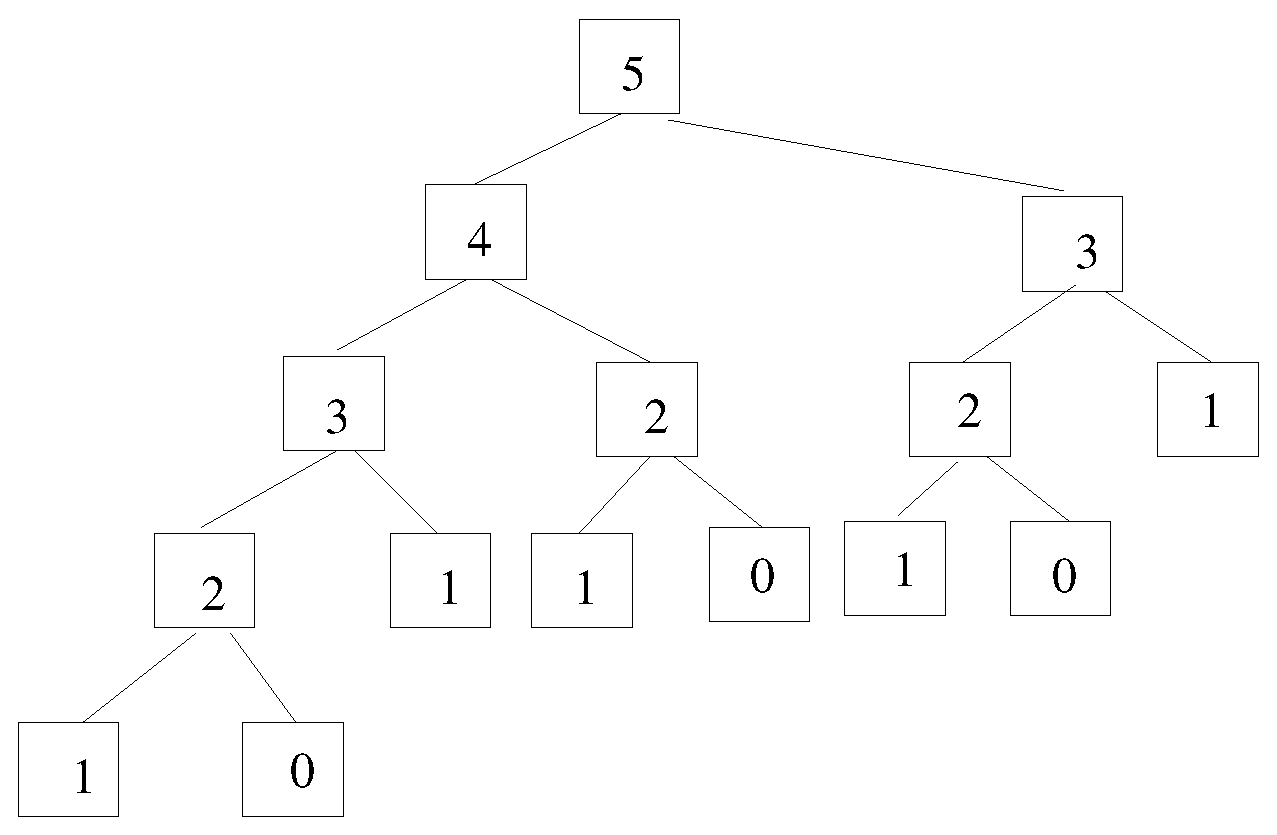
\includegraphics{fib-tree}}
\end{center}
\end{figure}

Note there is quite a bit of wasted work in this computation.
\texttt{fibonacci}(3) is computed twice throughout the tree, and
\texttt{fibonacci}(2) is computed three times.  When computing
\texttt{fibonacci}(n) for larger $n$, in fact many values are
repeatedly computed an exponentially large number of times (recall
that in Lab 5 we showed that the code above takes
$O(((1+\sqrt{5})/2)^n) \approx O(1.618^n)$ time to compute
\texttt{fibonacci}(n)).

Now here's an implementation of \texttt{fibonacci} using memoization.

\begin{verbatim}
def memoizedFibonacci(n, memory):
    if n<2:
        return 1
    if memory[n] != -1:
        return memory[n]
    memory[n] = memoizedFibonacci(n-1, memory) + memoizedFibonacci(n-2,memory)
    return memory[n]

def fibonacci(n):
    # memory[i] contains the answer we've already computed for
    # fibonacci(i), where it's -1 if we haven't computed it yet
    memory = []
    for i in xrange(n+1):
        memory += [-1]
    return memoizedFibonacci(n, memory)
\end{verbatim}

The above code takes only $O(n)$ time to compute \texttt{fibonacci}(n)
using just $O(n)$ additional memory.  There is a big difference
between $O(n)$ time and $O(1.618^n)$ time for even fairly small $n$.
For example, when $n=50$, $1.618^n$ is almost thirty billion.

Here's what the recursion tree
looks like for the new memoized implementation.

\begin{figure}[!!h]
\begin{center}
\scalebox{0.4}{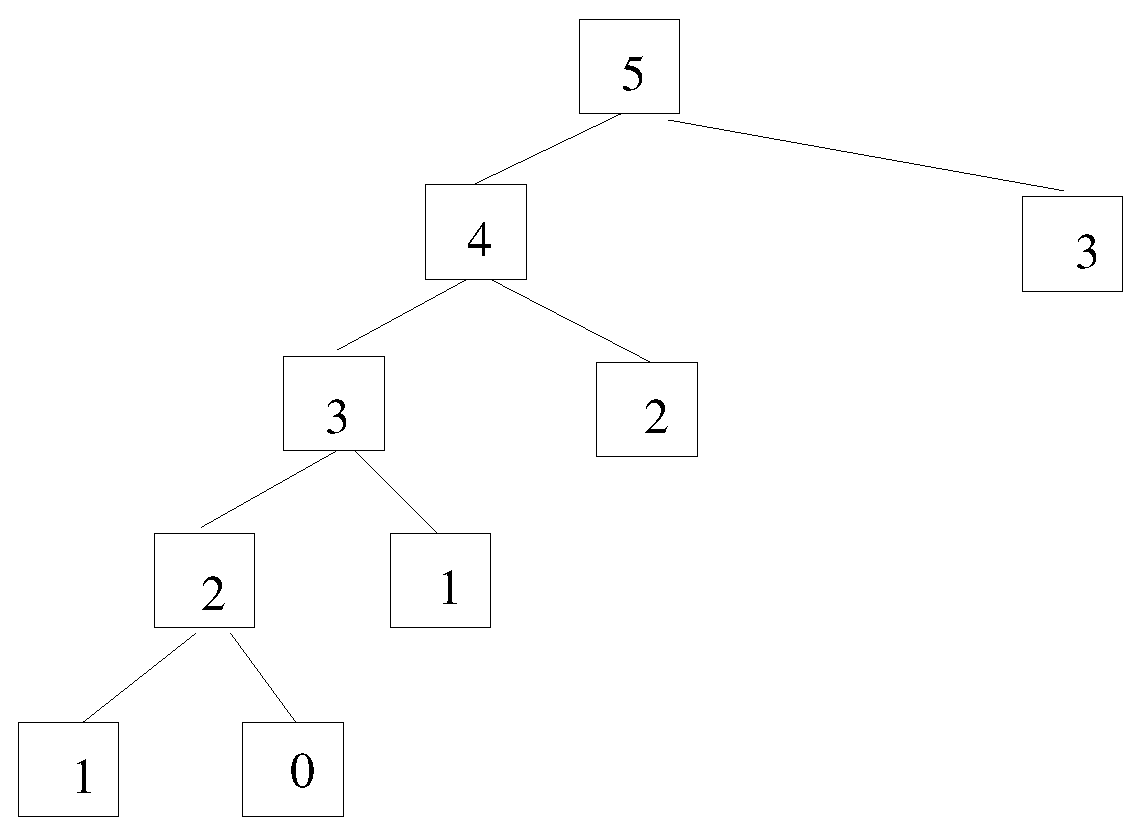
\includegraphics{memoized-tree}}
\end{center}
\end{figure}

For general $n$, the tree just looks like a long path going down the
left side, with one node hanging off the right side of every node.  In
general, there are less than $2n$ calls to the \texttt{fibonacci}
function throughout the recursion tree.

Another good example of dynamic programming is making change.  In the
US coin system, and also formerly in Ethiopia, there were coins for 1
cent, 5 cents, 10 cents, 25 cents, and 50 cents.  Suppose someone
gives you an amount and asks you to make change, how do you do it?
For example, what if they want you to make change for 88 cents?
You could give them 88 1-cent pieces, but that would be annoying.  You
could also give 17 5-cent pieces and 3 1-cent pieces, but that is
still kind of annoying.
Instead, usually we keep giving the largest coin we can until it's too
big,
then move to the next largest coin, etc.  For example, with 88 cents
we would first give a 50-cent piece, then a 25, then a 10, then three
3's, thus altogether giving 6 coins.  In fact for the value 88 cents,
making change in 6 coins is the best possible, and in fact this
approach of always giving the biggest coin first will always make
change using the least number of coins.

However, if we switch to another country which might have a different
coin system, this approach isn't always the best possible.  For
example, consider a country that has coins with the following
values: 1, 4, 5, and 10 cents.  Then, the strategy of giving the
highest value coin first would give 5+1+1+1 (4 coins) to make change
for 8 cents, whereas it's possible to do it with 2 coins (4+4).

Suppose we want to implement a function \texttt{makeChange}(n, L) as
follows.  n is some value we want to make change for, in cents, and L
is a list of values of all the different types of coins that exist in
our country.  The return value of \texttt{makeChange} should be the
minimum number of coins needed to make change for n cents.  We can
implement it recursively.

\begin{verbatim}
# if we can't make change for n cents using L, returns -2
def makeChange(n, L):
    if n==0:
        return 0
    # if possible to make change for n, the answer is definitely less
    # than n + 1
    answer = n + 1
    for x in L:
        if x <= n:
            val = makeChange(n-x, L)
            if val != -2:
                answer = min(answer, 1 + val)
    if answer == n + 1:
        answer = -2
    return answer
\end{verbatim}

The above code though runs quite slowly.  In fact, it's not too hard
to convince yourself that you can make it take exponential time in the
value $n$.  You
can speed it up, however, with memoization.

\begin{verbatim}
def memoizedMakeChange(n, L, memory):
    if n==0:
        return 0
    if memory[n] != -1:
        return memory[n]
    # if possible to make change for n, the answer is definitely less
    # than n + 1
    answer = n + 1
    for x in L:
        if x <= n:
            val = memoizedMakeChange(n-x, L, memory)
            if val != -2:
                answer = min(answer, 1 + val)
    if answer == n + 1:
        answer = -2
    memory[n] = answer
    return memory[n]

# if we can't make change for n cents using L, returns -2
def makeChange(n, L):
    # memory[i] contains the answer we've already computed to
    # make change for i cents, where it's -1 if we haven't computed it
    # yet. if we can't make change for n cents, we put -2 as the
    # value.
    memory = []
    for i in xrange(n+1):
        memory += [-1]    
    return memoizedMakeChange(n, L, memory)
\end{verbatim}

The above memoized version only takes $O(nm)$ time to figure out the
optimal number of coins to make change for $n$ cents, where $m$ is the
size of the list $L$.

\end{document}
